\documentclass[conference]{IEEEtran}
\IEEEoverridecommandlockouts
% The preceding line is only needed to identify funding in the first footnote. If that is unneeded, please comment it out.


%package
\usepackage{cite}
\usepackage{amsmath,amssymb,amsfonts}
\usepackage{algorithmic}
\usepackage{graphicx}
\usepackage{textcomp}
\usepackage{xcolor}
\usepackage{caption}
\usepackage{multicol}
\usepackage{blindtext}
\usepackage{stackengine}




%format
\def\BibTeX{{\rm B\kern-.05em{\sc i\kern-.025em b}\kern-.08em
    T\kern-.1667em\lower.7ex\hbox{E}\kern-.125emX}}
\begin{document}


%title
\title{After ARC : Consideration about Self-Tuning \\
{\footnotesize \textsuperscript}
\thanks{Advanced Operating System Term-Project}
}

\author{\IEEEauthorblockN{Jaehwan Jeong}
\IEEEauthorblockA{\textit{Department of Computer Science and Engineering} \\
\textit{Seoul Nat'l Univ, Real-Time Ubiquitous Systems Lab}\\
Seoul, Korea \\
jhjeong@rubis.snu.ac.kr}
\and
\IEEEauthorblockN{Tackhee Lee}
\IEEEauthorblockA{\textit{Department of Computer Science and Engineering} \\
\textit{Seoul Nat'l Univ, 3D Modeling and Processing Lab}\\
Seoul, Korea \\
thlee@3map.snu.ac.kr}
}



\maketitle

\begin{abstract}
This paper precisely speculates the probable enhancement of the adaptive replacement cache called ARC. More specifically, this paper introduces 3 tunable parameters which was fixed in previous adaptive replacment cache. We logically show the reasonable description that each parameter has  potential increase factor for the hit ratio of disk cache. We collected several traces that are widely-used in research-area for effective evaluation in terms of practicality.   
Conclusionally, This paper aims at finding 1)effectiveness of ARC is still valid in current days 2)our speculation called ``After-ARC" is reasonable. In order to find 1) and 2),  We evaluate ARC and ``After-ARC" with real-world benchmarks disk traces. Experimental results show that ARC is still valid in currently used benchmarks and our speculation ``After ARC" shows some interesting findings through results compare to ARC. 

\end{abstract}

\vspace{0.3cm}
\begin{IEEEkeywords}
Storage management-Secondary Storage, Cache Replacement Policy, Disk Cache, Adaptive Replacement Cache
\end{IEEEkeywords}

\section{Introduction}
Caching is one of the oldest and most fundamental metaphor in modern computing. The main problem of cache management is to design a replacement policy that maximizes the hit rate measured over a very long trace subject to the important practical constraints of minimizing the computational and space overhead involved in implementing the policy. Generally, CPU cache, its replacement policy implementation is limited to be simple due to the hardware-bounded constraints. e.g. logic-circuit design, processor support, cache-associativity, etc. However, for disk cache, such constraints are normally relaxed compared to CPU cache. i.e. there exists a chance to improve the hit ratio by developing a good cache replacement policy. From 1960s to 2000s, many research paper has been published to solve this problem, But a well-known, folklore algorithm, called LRU(Least Recently Used)~\cite{lru} showed a better performance by either hit ratio or tuning fashion. Even though there were some policies~\cite{lrfu},~\cite{mq} that show better hit ratio than LRU, they have critical weak points that they can outperform than LRU when some tunable paramter is fixed with some value. The existence of tuning-parameter seized them to overcome LRU policy due to the diversity of workload and computing environments since the value of paramter in each policy is highly depended on the workloads. e.g. database queries. 
To cope with this tuning-constraints, a novel cache replacement policy for disk cache called ARC(Adaptive Replacement Cache)~\cite{arc} has been published in 2003. Unlike other policies, ARC has no tunable parameters since it adaptively changes the parameters itself during its execution by its learning rate. They showed significant improvement compared to LRU with respect to both hit ratio and tuning-constraints. Accordingly, ARC and its variants have been widely used in storage system nowadays. e.g. IBM storage controller DS6000, ZFS file system~\cite{zfs}, PostgreSQL~\cite{postgresql}, VMware's vSAN~\cite{vsan}. 

Although the author of ARC~\cite{arc} claims that it is "self-tunable", However, in our point of view, there still exists some tunable parameters. First, they use initial value of $p$ as 0(which is the size of LRU portion in cache), but there's no guarantee that it is optimal for all workloads. Second, when they encounter phantom cache hit(i.e. actually miss, but exists in ghost cache), they use learning rate to increase/decrease size of LRU-LFU~\cite{lru} portion respectively or vice versa. However, there is no proof that the value of learning rate is reasonable for all workloads. Lastly, they limit the maximum size of $p$ as the cache size in ARC. However, this might loose full utilization of using ghost cache when they encountered a LRU-intensive workload. To investigate these conjectures, We first precisely speculate this observation. Second, we evaluate the hit-ratio of our ``After-ARC" variation compared to original ARC on real-life benchmark disk I/O traces. Since various second-storages e.g. Flash-memory, SSD(Solid State Drive) have emerged today, it is not reasonable for only measuring the hit ratio of the disk cache. However, this consideration is beyond the scope of this paper. We only aim at comparing our proposed variation of ARC is valid compared to original ARC. In terms of that, our evaluation is still valid. Additionally, we verify that ARC is still effective on the workloads that we use these days because it has been 16 years passed since ARC has been published and there have been a lot of changes on I/O patterns in several workloads. Our experimental results say that proposed speculation can be used to improve the hit ratio of the cache and ARC still derives efficient hit ratio for the disk cache.

This paper is organized as follows. In Section 2, we survey related works. Then, Section 3 briefly explains the idea of adapative cache replacement policy which we want to precisely  evaluate in terms of "self-tunable". In Section 4, we first explain our target traces i.e. real-life benchmarks that is widely used in research-area. And we also briefly describe about our simulation environment, and evaluates the experimental results. In Section 6, we discuss about the correctness of our consideration based on some interesting experimental results. Finally, Section 7 concludes the paper.


\vspace{0.2cm}
\section{Related Works}

For cache replacement policy, it is well-known that Belady's MIN~\cite{belady} algorithm is offline optimal in terms of hit ratio. Belady's MIN replaces the page that has the greatest distance. The policy MIN provides an upper bound on the achievable hit ratio by any on-line policy.

\subsection{Recency}
The policy LRU~\cite{lru} always replaces the least recently used page. LRU has several advantages, for example, it is simple to implement and responds well to changes in the underlying SDD(Stack Depth Distribution) model. However, it does not capture frequency. That is, in the long run, that each page is equally likely to be referenced and that therefore the model is useful for treating the clustering effect of locality but not the nonuniform page referencing. However, LRU still dominates among cache replacement policies because it is simple to implement and shows quite-good performance for all workloads.


\subsection{Frequency}
The Independent Reference Model(IRM) provides a workload characterization that captures the notion of frequency. Specifically, IRM assumes that each page reference is drawn in an independent fashion from a fixed distribution over the set of all pages in the auxiliary memory. The LFU~\cite{lru} captures frequency but it has several drawbacks. It requires logarithmic implementation complexity in cache size, pays almost no attention to recent history, and does not adapt well to changing access patterns since it accumulates stale pages with high frequency counts that may no longer be useful.

\subsection{Combining Recency and Frequency}
Several algorithms has been published to capture both recency and frequency. For example, FBR(Frequency-Based Replacement)~\cite{fbr} policy maintains a LRU list, but divides it into three sections : new, middle, and old. The key idea known as factoring out locality was that if the hit page was in the new section then the reference count is not incremented. On a cache miss, the page in the old section with the smallest reference count is replaced. Drawbacks of FBR is that to prevent cache poluution due to stale pages with high reference count but no recent usage the algorithm must periodically resize all the reference counts. The algorithm also has several tunable parameters, namely, the sizes of all three sections, and some other parameteres $C_{max}$ and $A_{max}$ that control periodic resizing. Another example, LRFU(Least Recently/Frequently Used) policy ~\cite{lrfu} subsumes LRU and LFU. Main difference between LRFU and FBR is that LRFU frequently weights each page's age more than FBR, that is, LRFU weights each page's age on every page access, but FBR periodically resizes the page's age. Also, LRFU has tunable parameter $\lambda$ and the performance of LRFU highly depends on $\lambda$. Now, we introduce ARC~\cite{arc} in Section III. More algorithm exists such as LARC~\cite{larc}, SARC~\cite{sarc}, CFLRU~\cite{cflru}, AIP~\cite{aip}, RRIP~\cite{rrip}, and etc. However, it is beyond the scope of this paper. If interested, refer these research papers.










\section{Brief Review of ARC}

\begin{figure}[t]
 \centering
 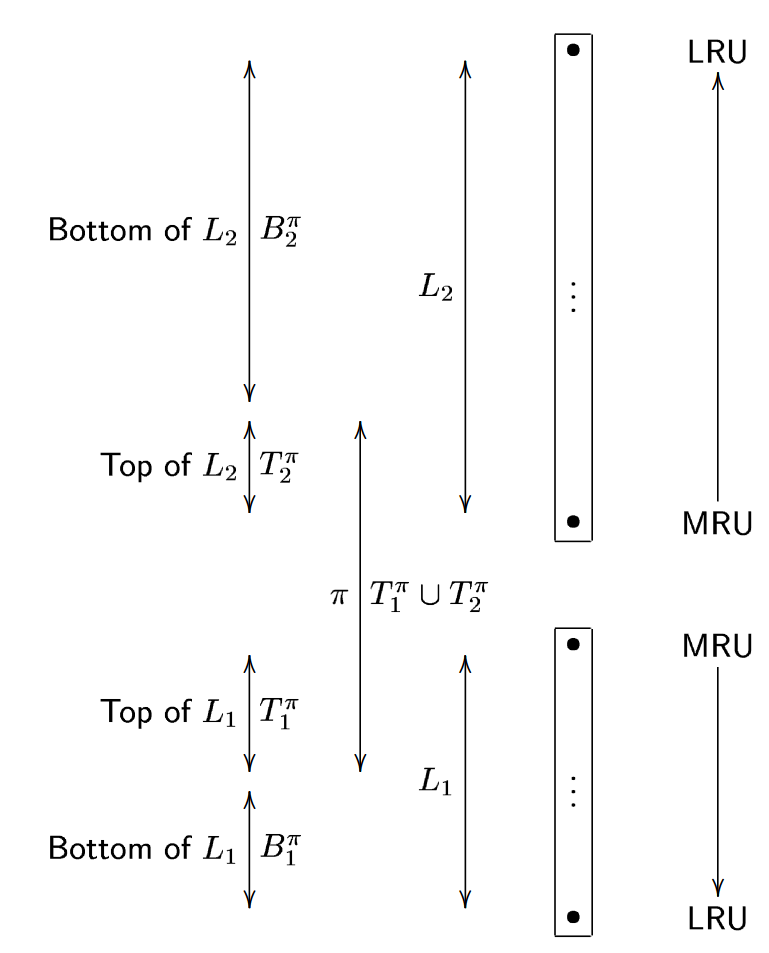
\includegraphics[width=8cm,height=9cm]{Figures/arc.PNG}
 \captionsetup[figure]{font=normalsize}
 \caption{General structure of generic cache replacement policy}
 \vspace{-0.5cm}
 \label{fig:arc}
\end{figure}


We now show brief explanation about ARC~\cite{arc}. Main difference between ARC and the other policies is that ARC adaptively changes its paramter. More specifically, the paramter of ARC is defined as the size of LRU/LFU portion within cache. We will show how it adaptively changes its size during runtime through Section A to C. 

\subsection{LRU and LFU}
 Many researchers attempted to make an algorithm that captures both recency and frequency. Since almost the whole workloads has both locality and frequency. So in order to the derive high hit ratio of the cache, For researchers, it was a fate to capture those properties together. However, all of them had critical drawbacks that they have to assign some value to their parameters in order to derive higher hit ratio, and it highly depends on the access pattern of certain workloads. Before describing ARC, We show a generic cache replacement policy which was used in ARC. Figure~\ref{fig:arc} shows the general structure of generic cache replacement policy. \\
 This policy ensures that following invariants will always hold:\\
 \vspace{-0.2cm}
 \begin{center}
 $ 0 \leq |L_1| + |L_2| \leq 2c$, $ 0 \leq |L_1| \leq c$, $0\leq |L_2| \leq 2c.$
 \end{center}

 
 Also, in below conditions A.1-5 hold for generic cache replacement policy.
 \vspace{0.2cm}
 \begin{itemize}
     \item A.1. The lists $T_1^\pi$ and $B_1^\pi$ are disjoint and, also, the lists $T_2^\pi$ and $B_2^\pi$ are disjoint, and 
     $L_1$ = $T_1^\pi$ $\cup$ $B_1^\pi$ and $L_2$ = $T_2^\pi$ $\cup$ $B_2^\pi$.
 \end{itemize}

\begin{itemize}
    \item A.2 If $|L_1 \cup L_2| < c$, then both $B_1^\pi$ and $B_2^\pi$ are empty.
\end{itemize}

\begin{itemize}
    \item A.3 If $|L_1 \cup L_2 | \geq c$, then, together $T_1^\pi$ and $T_2^\pi$ contain exactly c pages. 
\end{itemize}

\begin{itemize}
    \item A.4 Either $T_1^\pi$(resp. $T_2^\pi$) or $B_1^\pi$ (resp. $B_2^\pi$) is empty, or the LRU page in $T_1^\pi$ (resp. $T_2^\pi$) is more recent than the mRU page in $B_1^\pi$ (resp.$B_2^\pi$).
\end{itemize}

\begin{itemize}
    \item A.5 For all traces and at each time, $T_1^\pi \cup T_2^\pi$ will contain exactly those pages that would be maintained in cache by the policy $\pi(c)$.
\end{itemize}

 Key concept of this cache replacement policy is that $L_1$ holds pages that requested only once and $L_2$ holds pages that requested more than once. $|T_1 \cup T_2|$ is the actual cache and it keeps exactly the same size as cache size $c$. Compared to $T_1$ and $T_2$, $B_1$ and $B_2$ is used for the cache replacement management. i.e. ghost cache. In Figure~\ref{fig:arc}, the ghost cache size is set to $2c$.

\subsection{Ghost Cache}
In ARC, they maintain a larger cache directory than that is needed to support the underlying cache. Such directories are known as a shadow cache or as a ghost cache. Previously, ghost caches have been employed in a number of cache replacement algorithms. ARC uses this ghost cache for adaptively determine the size of $T_1$ and $T_2$, $B_1$ and $B_2$ respectively. 

\subsection{Adaptive Replacement Cache}


\begin{figure}[t]
 \centering
 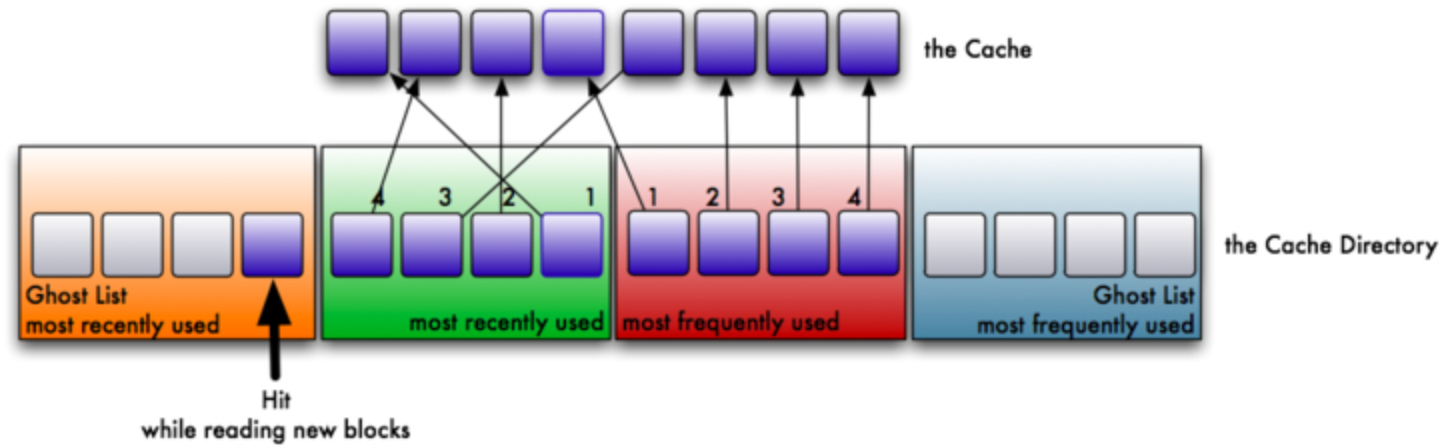
\includegraphics[width=9cm,height=5cm]{Figures/phantom_cache_hit.PNG}
 \captionsetup[figure]{font=normalsize}
 \caption{A situation that phantom hit occurs}
 \vspace{-0.5cm}
 \label{fig:phantom_hit}
\end{figure}


\begin{figure}[t]
 \centering
 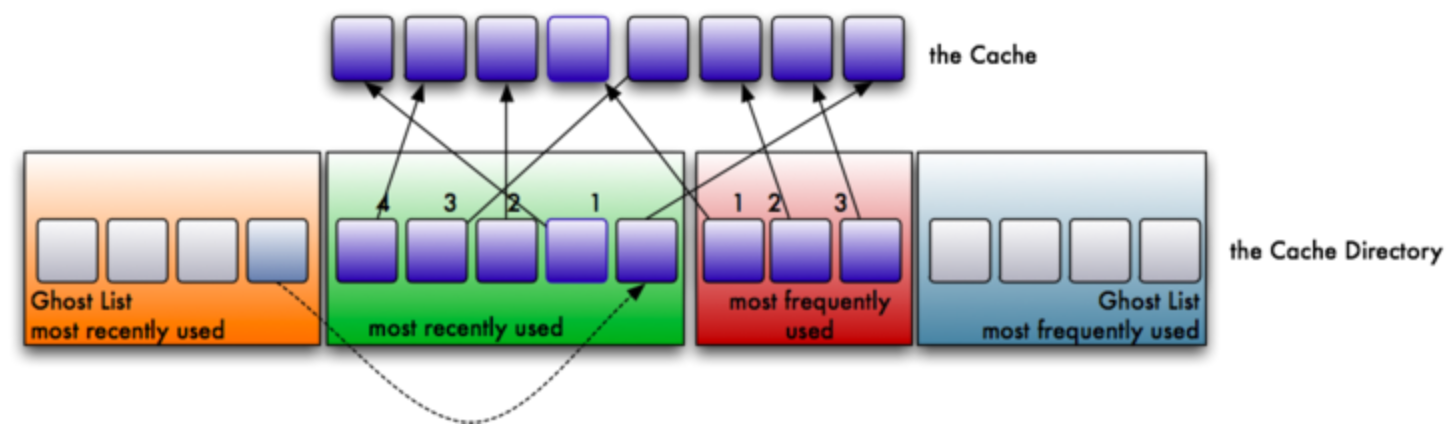
\includegraphics[width=9cm,height=5cm]{Figures/phantom_cache_hit_after.png}
 \captionsetup[figure]{font=normalsize}
 \caption{Adaptive resizing from ARC}
 \vspace{-0.5cm}
 \label{fig:phatom_hit_after}
\end{figure}


The main idea of ARC is quite simple. They maintain a ghost list i.e. $B_1$ and $B_2$.  when they encountered the cache miss, they treat it as a actual-miss or phantom-hit (i.e. hit on $B_1$ or $B_2$). So if phantom-hit occurs, then ARC adaptively resizes the portion of $T_1$(i.e. phantom hit on $B_1$) or $T_2$(phantom hit on $B_2$). This is not actually accurate because some exceptions exist. Note that we describe brief the concept of ARC so if interested in 
more detailed algorithm, See [Fig 4 in~\cite{arc}]. From Figure 2 and Figure 3, we can see the adaptive resizing of ARC, In Figure ~\ref{fig:phantom_hit}, We can see that actual cache size is 8. and ghost cache size is 16. Initial situation is same as following, $|T_1|=4, |B_1|=4, |T_2|=4, |B_2|=4$. Then phantom-hit occurs on $B_1$, So from that, ARC resizes the $|T_1|$ from $4$ to $5$, and $|T_2|$ from $4$ to $3$. $|B_1|$ and $|B_2|$ has same value in Figure 2 and 3. Note that this is a example for explaining ARC and it is not exactly same as ARC(i.e. a variant from ZFS-ARC) but the main idea(i.e. adaptive replacement) is same. Actually, various cases happen when a phantom-hit or actual miss occurs. See [Fig 4 in ~\cite{arc}]. 



\section{Consideration about "self-tuning"}

In ARC, they actually assign $p$ i.e. the maximum length of $|T_1|$ as 0 before starting, and they limits the maximum size of $p$ with $c$ i.e. actual cache size. Also, when phantom-hit occurs on $B_1$, they increase the size of $T_1$ from the following equation. 

\vspace{0.3cm}
\scalebox{0.9}{
\begin{equation}\label{eq1}

p = min\{p+\delta_{1}, c\}, 
\, \text{where} \; 
\delta_1 = \begin{cases} 1           & \text{if} |B_1| \geq |B_2|  \\
                         |B_2|/|B_1| & \text{otherwise.}

\end{cases} 
\end{equation}
}

\vspace{0.2cm}
When phantom-hit occurs on $B_2$, they decrease the size of $T_1$ like Eq.(1), but differs with ``+" to ``-", and the inequality on Eq. (1) reverses from $\geq$ to $\leq$. Other things are exactly same. For simplicity, from now on, we will mark learning rate value as $\delta$ no matter whether phantom-hit occurs on $B_1$ or $B_2$. Eq. (1) intuitively involves the intention that if the following inequality $|B_2| \geq |B_1|$ holds, then there will be a lot of chances for encountering phantom-hit on $B_1$ again. So in order to avoid that situation again, ARC increase the size of $p$ as $|B_2|/|B_1|$ not 1, and it is called learning rate.

\subsection{Initial Value of $p$}
In ARC, it starts algorithm with initial value $p$ as 0, However, assigning $p$ with value 0 does not guarantee that it is the best-choice. $p$ indicates that ARC tries to re-size the length of $T_1$ to $p$ as much as possible. Although ARC will adaptively change the parameter $p$ during its runtime, initial value of $p$ still can affect the hit ratio of the workload. So, we aim to evaluate the effectiveness of initial value $p$ in terms of portion on hit ratio and the value itself by changing initial value of $p$   


\subsection{Limit value of $p$}
In ARC, it limits the maximum size of $p$ as c. This indicates that even though a certain workload is highly LRU-intensive, ARC cannot increase the size of LRU portion i.e. $|L_1|$ to $2c$. We guess that author's intention is 1)balancing the portion of LRU and LFU to 1:1. 2)It is meaningless because if phantom-hit occurs, then that page always goes to the MRU position of $T_2$, so it can be covered by $T_2$ even for the highly LRU-intensive workloads too. Although this is acceptable, There's no right answer on that. So, we aim to evaluate the effectiveness of the maximum value of $p$ in terms of LRU-LFU portion by changing the maximum value of $p$. 


\subsection{Learning Rate}
In ARC, if phantom-hit occurs, then they increase the size of $p$ following as Eq. (1). Learning rate i.e. Eq. (1) indicates that ARC prefers to avoid the phantom-hit on the same hidden list i.e. $B_1$ or $B_2$. However, the value of learning rate, $\delta$ does not guarantee that it is the best-choice. So, we aim to evaluate the effectiveness of the learning rate by changing $\delta$.

More specifically, First, we vary initial value of $p$ as 0, $\frac{c}{2}$ and $c$. Second, we vary limit value of $p$ as c, $\frac{1}{3}c$ $\frac{2}{3}c$, $\frac{4}{3}c$ and $\frac{5}{3}c$. Lastly, we vary the learning rate $\delta$ as $\pm2$, $\delta$, $\log_2{\delta}$ and $2^\delta$. Experimental results are shown in Section V.








\section{Evaluation}



\subsection{Collecting Benchmark Traces}\label{Trace}

Table I summarizes various traces that we used in this paper. These traces mainly include 3 traces. FIU Traces~\cite{fiu}, MS Production server traces~\cite{microsoft}, MS Enterprise traces~\cite{microsoft}. We use these traces because it is widely used for second storage research area, also it is available for free via SNIA/IOTTA(Storage Networking Industry Association's Input/Output Traces, Tools, and Analysis)~\cite{snia}.



\begin{table}[h]

\begin{center}
\begin{tabular}{|c|c|c|}
\hline
\textbf{Trace Name}&\textbf{Number of Request} & \textbf{Unique Pages} \\
\cline{2-3} 
\hline
Exch   & 77304451 & 21724991    \\ 
\hline
DAP-DS & 11184349 & 5092722   \\
MSN    & 11115258 & 7209398   \\
RAD-AS & 5529468 & 3323691   \\
RAD-ES & 39405995 & 20608323 \\        
\hline
HOMES  & 21163638  & 4760647 \\
WEB-VM & 14294158 & 549174 \\
MAIL   & 14010588 & 1913909 \\

\hline
\end{tabular}
\label{tab1}
\end{center}
\caption{Summary of disk traces}
\end{table}

For all traces, the page size is 4KB. Also, all hit ratios reported in this paper are cold start. We will report hit ratios in percentages (\%). We briefly explain the characteristics of each disk traces on the following subsections from 1) to 3). For all traces, We first append all logs of it and parsed disk I/O pattern from them.
\vspace{0.3cm}
\subsubsection{Traces 1} MS Enterprise traces
 

\begin{itemize}
\item Exchange server (\textbf{Exch}) \\
 The Microsoft Exchange 2007 SP1 server is a mail server
for 5000 corporate users. It is a 4-socket, dual-core system
with 4 GB of memory. The storage consists of two 146 GB
SAS drives in a RAID-1 configuration, six data arrays of
fourteen 146 GB SAS drives, and two log arrays of eight
146 GB SAS drives configured as RAID-10. One trace
covers a 5-hour peak load period on a weekday afternoon.
Another trace covers a 24-hour weekday period. The traces
are broken into 15-minute intervals. 
\end{itemize}

\subsubsection{Traces 2} MS Production Server traces

\begin{itemize}
\item Display Ads Platform data and payload servers(\textbf{DAP}) \\
 The purpose of the data server (\textbf{DS}) is to be a caching tier
between the front-end server and the payload server (PS). A
front-end server makes an advertisement request with a user
id to the \textbf{DS}. The \textbf{DS} looks up the user id in the cache,
appends any information available for that user to the
request, and passes the request to the PS. The PS is
responsible for ad selection. The traces from the DS and PS
cover a 24-hour period and are broken into 30-minute
intervals.
\end{itemize}

\begin{itemize}
\item MSN storage metadata and file servers (\textbf{MSN}) \\
 The CFS server stores metadata information and blobs correlating users to files stored on the back-end file server(\textbf{MSN}). The \textbf{MSN} provides the files requested by CFS. The servers are used by serval Live data services. The traces from the CRS and \textbf{MSN} cover a 6-hour period and are borken into 10-minute intervals.



\end{itemize}



\begin{itemize}
\item RADIUS authentication and back-end server (\textbf{RAD}) \\
 The RADIUS authentication server (AS) is responsible for
worldwide corporate remote access and wireless
authentication. It runs the IPSec NAP scenario. Data comes
in via SQL replication on the back-end SQL server (\textbf{ES}).
The traces from the AS and \textbf{ES} cover an 18-hour period and
are broken into 1-hour intervals.
\end{itemize}



\subsubsection{Traces 3} FIU traces

\begin{table*}[th]
    \captionsetup{font=normalsize}
    \normalsize
    \centering
    
        \begin{tabular}{|c|c|c|c|c|c|c|c|c|}

\hline
 &\textbf{EXCH} & \textbf{DAP-DS} & \textbf{MSN} & \textbf{RAD-AS} & \textbf{RAD-ES} & \textbf{HOMES} & \textbf{WEB-VM} & \textbf{MAIL} \\
\hline
\cline 

$p=0$ &           $12.71$ & $3.59$ & $16.71$ & $22.19$ & $19.43$ & $59.28$ & $73.16$ & $54.61$   \\ 
\hline
$p=\frac{c}{2}$ & $12.88$ & $ 3.78$ & $16.53 $ & $22.42 $ & $20.64 $ & $58.81 $ & $70.71 $ & $53.65 $ \\ 
\hline
$p=c$ &           $12.65$ & $3.69$ & $15.77$ & $20.34$ & $19.57$ & $59.39$ & $73.13$ & $54.60$ \\ 
\hline
        \end{tabular}
\caption{Hit ratio as varying initial value $p$}
\end{table*}

\vspace{0.2cm}


\begin{table*}[th]
    \captionsetup{font=normalsize}
    \normalsize
    \centering
    
        \begin{tabular}{|c|c|c|c|c|c|c|c|c|}

\hline
 &\textbf{EXCH} & \textbf{DAP-DS} & \textbf{MSN} & \textbf{RAD-AS} & \textbf{RAD-ES} & \textbf{HOMES} & \textbf{WEB-VM} & \textbf{MAIL} \\
\hline
\cline 

$p_{max}=c$ &           $12.71$ & $3.59$ & $16.71$ & $22.19$ & $19.43$ & $59.28$ & $73.16$ & $54.61$   \\ [1ex]
\hline
$p_{max}=\frac{1}{3}c$ & $12.86$ & $2.84$ & $16.26$ & $19.59$ & $12.62$ & $ 56.18 $ & $67.59$ & $54.26$ \\ [1ex]
\hline
$p_{max}=\frac{2}{3}c$ & $12.88$ & $3.45$ & $18.07$ & $21.58$ & $20.62$ & $59.05$ & $74.60$ & $55.81$   \\ [1ex]
\hline
$p_{max}=\frac{4}{3}c$ & $12.85$ & $3.56$ & $9.84$ & $19.09$ & $20.91$ & $49.87$ & $79.47$ & $49.87$   \\ [1ex]
\hline
$p_{max}=\frac{5}{3}c$ & $12.48$ & $3.37$ & $7.01$ & $15.80$ & $19.77$ & $42.87$ & $78.90$ & $42.87$   \\ [1ex]
\hline

        \end{tabular}
\caption{Hit ratio as varying limit value of $p$}
\end{table*}






\begin{table*}[th]
    \captionsetup{font=normalsize}
    \normalsize
    \centering
    
        \begin{tabular}{|c|c|c|c|c|c|c|c|c|}

\hline
 &\textbf{EXCH} & \textbf{DAP-DS} & \textbf{MSN} & \textbf{RAD-AS} & \textbf{RAD-ES} & \textbf{HOMES} & \textbf{WEB-VM} & \textbf{MAIL} \\
\hline
\cline 

ORIGIN & $12.71$ & $3.59$ & $16.71$ & $22.19$ & $19.43$ & $59.28$ & $73.16$ & $54.61$   \\ 
\hline
CONST & $12.79$ & $3.64$ & $15.81$ & $21.32$ & $20.60$ & $ 58.82 $ & $ 71.94 $ & $ 52.87 $ \\ 
\hline
LOG &   $12.71$ & $ 3.57 $ & $ 16.26 $ & $ 21.61 $ & $19.44$ & $ 59.22 $ & $ 73.45 $ & $53.91$   \\
\hline
EXP &   $12.88$ & $ 3.72 $ & $ 16.37 $ & $ 22.47 $ & $ 20.60$ & $ 58.72 $ & $ 70.63 $ & $ 53.59 $   \\ 
\hline


        \end{tabular}
\caption{Hit ratio as varying the value of learning rate \delta}
\end{table*}




\begin{itemize}
\item Virtual machine running 2 web-servers (\textbf{WEB-VM}) \\
The \textbf{WEB-VM} workload is collected from a virtualized system that hosts two CS
department web-servers, one hosting the department's online course management system
and the other hosting the department's web-based email access portal. the local virtual disks
which were traced only hosted root partitions containing the OS distribution, while the http data for these web-servers reside on a network-attached storage.
\end{itemize}

\begin{itemize}
\item Mail-Server from FIU (\textbf{MAIL}) \\
The \textbf{MAIL} workload serves user INBOXes for the entire Computer Science department at FIU(Florida International University).
\end{itemize}

\begin{itemize}
\item NFS server from FIU (\textbf{HOMES}) \\
The \textbf{HOMES} workload is that of a NFS server that serves the home directories of FIU's small-sized research group; activities represent those of a typical researcher consisting of software development, testing, and experimentation, the use of graph-plotting software, and technical document preparation.
\end{itemize}

To simulate the cache behaviours, we fix the disk cache size as 256MB. From fixing the disk cache size and page size, and collecting disk I/O traces, we run total 72 simulation by varying some tunable parameters as we mentioned in Section IV. 


\subsection{Experimental Result}\label{expresult}



\subsubsection{Experiment 1} Initial Value of $p$ \\
 As we mentioned in Section IV, we vary initial $p$ value as 0, $\frac{c}{2}$ and $c$. Table II shows the result hit ratio of each trace. The first column of the table represents the initial value of $p$. In case of $p=c$ which means the initial value of $p$ is $c$, only HOMES derives higher hit ratio compared with the other 2 cases. In case of $p=\frace{c}{2}$, EXCH,DAP-DS,RAD-AS and RAD-ES derives higher hit ratio compared with the other 2 cases. Maximum difference value among $p=0$ and $p=c$ appears as approx 3\% in WEB-VM. Normally, the gap among all 3 cases comes with the degree of $10^{-1}$. Conclusionally, there is no tendency with the initial value $p$ and the amount of standard deviation in Experiment 1 is normally negligible.
\vspace{0.2cm}

\subsubsection{Experiment 2} Limit Value of $p$ \\
We now vary the limit value of $p$ which means the maximum length of LRU portion as $\frac{1}{3}c$, $\frac{2}{3}c$, $c$, $\frac{4}{3}c$, $\frac{5}{3}c$. This intuitively indicates that the rate between LRU and LFU becomes 1:5, 1:2, 1:1, 2:1 and 5:1 since ARC uses ghost cache size as $2c$. Table III shows the result hit ratio of each trace. $p_{max}$ means that we fix the maximum size of $p$ as $p_{max}$. In case of $p_{max}=c$, DAP-DS, RAD-AS and HOMES derives the most highest hit ratio among them. In case of $p_{max}=\frac{2}{3}c$, EXCH, MSN and MAIL derives the most highest hit ratio. In case of $p_{max}=\frac{4}{3}c$, RAD-ES and WEB-VM derives the most highest hit ratio. We can expect that these EXCH, MSN and MAIL traces are more LFU-biased workloads since ARC can expand its maximum size for LRU portion maximum to $\frac{2}{3}c$. i.e. $L_1$. On the contrary to this, RAD-RES and WEB-VM traces are more LRU-biased workloads since ARC can expand to its maximum size for LRU portion maximum to $\frac{4}{3}c$. i.e. $L_1$. Lastly, DAP-DS,RAD-AS, and HOMES are balanced workload between LRU and LFU since they derive the most highest ratio in case, $p_{max}=c$. Note that we are dealing with the cache directory size i.e. ghost cache size not the actual size of the cache. Interesting finding is that for all of them, the worst-case hit ratio configurations always appear when $p_{max}$ is either $\frac{1}{3}c$ or $\frac{4}{3}c$. This intuitively indicates that since we forcibly suppress the size of $p$ into $\frac{1}{3}c$ or $\frac{4}{3}c$, it cannot freely enjoy the freedom of adaptive replacement. At first, we anticipated that more LRU/LFU-intesive workload can get more higher ratio on these configurations. However, this tendency tells us that real-world workloads are not purely 100\% biased to LRU or LFU, in which, is the mixture type of LRU and LFU. Also, we can see original-ARC always performs above the average with all simulation cases. In summary, ARC performs well with respect to the adaptive replacement. Also, there exists some cases that performs better than ARC when we assign the maximum value $p$ with the bounded range from $c$.


\vspace{0.2cm}
\subsubsection{Experiment 3} Learning Rate \\
In this simulation experiment, We now vary the learning rate value with the ORIGIN, CONST, LOG and EXP. ORIGIN denotes that the value of learning rate is same as ARC~\cite{arc}. CONST denotes that in contrary to Eq. (1), if we encountered the phantom-hit, then we always increase/decrease the size of $T_1$ as 2.  LOG denotes that the value of learning rate is $\log_2{\delta}$. Note that $\delta$ denotes the original learning rate value of ARC. Lastly, EXP denotes that the value of learning rate is $2^\delta$. Table IV shows the hit ratio of each traces. For MSN, HOMES, and MAIL, \textbf{ORIGIN} derives the most highest hit ratio among 4 configurations. For WEB-VM, \textbf{LOG} derives the most highest. For EXCH, DAP-DS, RAD-AS, and RAD-ES, \textbf{EXP} derives the most highest. \textbf{LOG} indicates that it smoothly does re-sizing compared to \textbf{ORIGIN}. Similarly, \textbf{EXP} indicates that it roughly does re-sizing compared to \textbf{ORIGIN}. We denote these trace sets as 1) Group 1 : EXCH, DAP-PS, RAD-AS, RAD-ES 2) Group 2: MSN, HOMES, MAIL, 3) Group 3 : WEB-VM. From Table IV, We can speculate the traces of Group 3 smoothly changes its I/O access pattern among three groups. Contrary to Group 3, we can speculate the traces of Group 1 roughly changes its I/O access pattern among three groups. Conclusionally, ARC(i.e. ORIGIN) performs well above the average for the all simulation cases. Also, in case of EXP, it performs better than ARC(i.e. ORIGIN) in 4 traces up to maximum 0.6\%. For the other 4 cases, EXP performs worse than ARC, but the difference between EXP and ARC(i.e. ORIGIN) is up to maximum 0.4\% except MAIL traces. We suggest that the exponential learning rate value is quite good-option based on the results in Table IV. 

Finally, we present our contributions. 1)We confirm that the effectiveness of ARC is still valid through real-life benchmark traces which is widely used in research-area nowadays. In Table III, ARC performs better than $p_{max}=\frac{5}{3}c$ up to maximum 17\% except RAD-ES and WEB-VM. $p_{max}=\frac{5}{3}c$ indicates that it behaves like LRU(not exactly LRU) since the portion of LRU is 5 times larger than the portion of LFU. With this result, we can say ARC performs better than LRU for the most of general workloads. 2)We investigate the authentic "self-tunablity" by performing Experiment 1 to 3. From Experiment 1, we confirmed that the change of initial value $p$ affects negligibly small amount on the hit ratio. In terms of initial value $p$, we can say ARC is self-tunable. From Experiment 2, we confirmed that the changes of limit value $p$ affect quite larger portion of the hit ratio. However, it is workload-dependent. Also, we verified when the limit value of $p$ gets smaller or bigger from $c$, it performs much worse on every workload. This indicates that if we balance the portion of LRU(i.e. $L_1$) and LFU(i.e. $L_2$) closer to 1:1, we can ensure that it will perform not the highest but the above average on a certain workload compare to other configurations. In short, the choice of $p$ to $c$ was best-choice.
From Experiment 3, we confirmed that the value of learning rate in ARC performs above the average on all traces. However, we also found that assigning the value of learning rate like \textbf{EXP} is also quite good-option. We insist that selecting the learning rate value like \textbf{EXP} gives much higher ratio on some workloads which dynamically changes its I/O access. And it also ensures that even if it does not perform than ARC, the gap between EXP and ARC are quite tolerable for that kind of workloads.





\section{Discussion}

About practicality, we cannot say it is practical since we does not consider the trend of the second-storages. e.g. Flash-Memory, SSD. Espeically for flash-memory, it involves the write amplification and wear-leveling due to P/E cycle which affects the life-cycle of flash memory. We only measured the hit ratio of the disk traces, However, we expect that there is some amplifications for disk operations due to garbage collection or wear-leveling. Despite of that, we investigate the validity of ARC in terms of 3 tunable parameters and find that 1) EXP is quite good-option, 2) ARC is still useful replacement policy in current-days workloads. If interested in second storage properties, refer these following research papers~\cite{ssd1},~\cite{ssd2},~\cite{cflru},~\cite{flash}.\\
About experiment, we collected about 30 traces. e.g. traces from SYSTOR17 Lee et al traces~\cite{systor17}, and other traces from ~\cite{microsoft} e.g. TPC-C, TPC-E, LM-TFE, WBS, DTRS, and etc. we spent about 4 days for parsing the disk I/O patterns of each trace. There was a lack of time for simulating all 30 traces within short days. So we only showed the simulation results for 8 traces. we spent about 8 hours for simulating those 8 traces. It would be more nice to measure the other 22 traces with the same configurations in Section V. Also, we fixed the size of disk cache as 256MB, but the size of disk cache in currently released servers varies from 128MB to even 2GB. We think that it would be also useful to simulate those traces with a much higher disk cache size. All sources used in this paper are freely available on our GitHub repository~\cite{opensource}. Note that even each parsed data was so big to upload at web-site, we omitted the actual/parsed traces. However, the code for parsing disk traces are available on web-site~\cite{opensource} and all actual traces are freely available on SNIA/IOTTA~\cite{snia}. For researchers who are interested in this paper, we anticipate that anyone can easily use our open-source code. Hopefully, it would be nice that our source could be used for the basis of the further research or implementation for ARC or variants of ARC.



\input{conclusion}



 





\bibliographystyle{IEEEtran}
\bibliography{archive}



\vspace{12pt}


\end{document}
